\section{Le 3b-1}

% \subsection*{(a)}
The code and figure generating 500 particles to represent the distribution with equal weight is as follows:
\begin{matlabcode}
N = 500;
w = 1/N + zeros(1,N);
for ii = 1:N
    x(ii) = normrnd(0,1) * w(ii);
end
[fx,xk]=ksdensity(x); 
\end{matlabcode}
% The data sample is shown in the following figure:
\begin{figure}[!h]
    \centering
    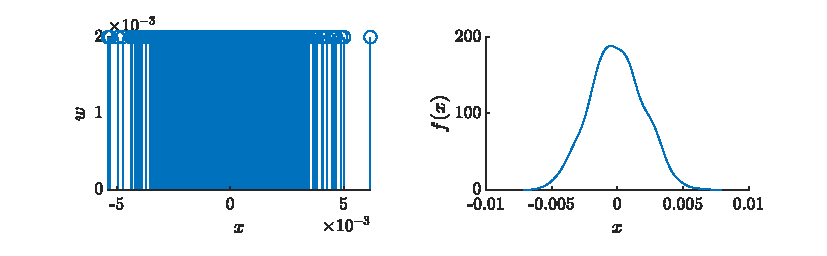
\includegraphics{figures/ex4_a.pdf}
\end{figure}

% \subsection*{(b)}

The particles from the previous exercise were used to compute new particles 
representing the distribution is shown in the figure below:
\begin{figure}[!h]
    \centering
    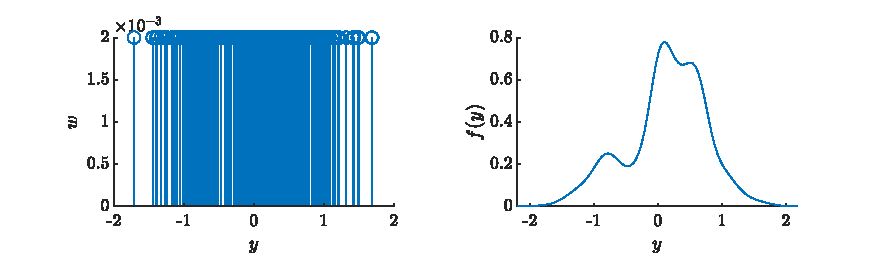
\includegraphics{figures/ex4_b.pdf}
\end{figure}
